%Dokumentklasse
\documentclass[a4paper,12pt]{scrreprt}
\usepackage[left= 2.5cm,right = 2cm, bottom = 4 cm]{geometry}
%\usepackage[onehalfspacing]{setspace}
% ============= Packages =============

% Dokumentinformationen
\usepackage[
	pdftitle={Titel der Abschlussarbeit},
	pdfsubject={},
	pdfauthor={Euer Name},
	pdfkeywords={}
	pdftex=true, 
	colorlinks=true,
 	breaklinks=true,
	citecolor=black,
	linkcolor=black,	
	menucolor=black,	
	urlcolor=black
]{hyperref}


% Standard Packages
\usepackage[utf8]{inputenc}
\usepackage[ngerman]{babel}
\usepackage[T1]{fontenc}
\usepackage{graphicx}
\graphicspath{{img/}}
\usepackage{fancyhdr}
\usepackage{lmodern}
\usepackage{color}
\usepackage{transparent}

% zusätzliche Schriftzeichen der American Mathematical Society
\usepackage{amsfonts}
\usepackage{amsmath}

% nicht einrücken nach Absatz
\setlength{\parindent}{0pt}


% ============= Kopf- und Fußzeile =============
\pagestyle{fancy}
%
\lhead{}
\chead{}
\rhead{\slshape \leftmark}
%%
\lfoot{}
\cfoot{}
\rfoot{\thepage}
%%
\renewcommand{\headrulewidth}{0.4pt}
\renewcommand{\footrulewidth}{0pt}

% ============= Package Einstellungen & Sonstiges ============= 

%Besondere Trennungen
\hyphenation{De-zi-mal-tren-nung St-rei-fen-licht-scan-nern}

%römische Aufzählungen mit \RM{Zahl}
\newcommand{\RM}[1]{\MakeUppercase{\romannumeral #1}}


% ============= Dokumentbeginn =============

\begin{document}

\pagestyle{empty}
\begin{center}
\begin{tabular}{p{\textwidth}}


\begin{center}

\includegraphics[scale=0.2]{img/logos.jpg}
\end{center}


\\

\begin{center}
\LARGE{\textsc{
Ein super toller Titel \\
}}
\end{center}

\\


\begin{center}
\large{Fakultät für Muster und Beispiele \\
der Hochschule Musterhausen \\}
\end{center}

\\

\begin{center}
\textbf{\Large{Abschlussarbeit}}
\end{center}



\begin{center}
vorgelegt von
\end{center}

\begin{center}
\large{\textbf{Max Mustermann}} \\
\small{geboren am 01.01.1900 in Musterhausen}
\end{center}

\begin{center}
\large{im Dezember 2014}
\end{center}

\\

\\

\begin{center}
\begin{tabular}{lll}
\textbf{Erstprüfer:} & & Prof. Dr. med. Dr.-Ing. M. Mustermann\\
\textbf{Zweitprüfer:} & &Prof. Dr.-Ing. F. Musterfrau\\
\end{tabular}
\end{center}

\end{tabular}
\end{center}

% \part im Inhaltsverzeichnis nicht nummerieren
\makeatletter
\let\partbackup\l@part
\renewcommand*\l@part[2]{\partbackup{#1}{}}

%Seitennummerierung neu beginnen, Zahlen [arabic], röm.Zahlen [roman,Roman], Buchstaben [alph,Alph]
\pagenumbering{Roman}

\newpage
\addsec{Eidesstattliche Erklärung}
\label{erklaerung}

Hiermit versichere ich, die vorliegende Studienarbeit selbstständig und nur unter Verwendung der von mir angegebenen Quellen und Hilfsmittel verfasst zu haben. Sowohl inhaltlich als auch wörtlich entnommene Inhalte wurden als solche kenntlich gemacht. Die Arbeit hat in dieser oder vergleichbarer Form noch keinem anderem Prüfungsgremium vorgelegen. \\
\\[1.5cm]
Datum:	\hrulefill\enspace Unterschrift: \hrulefill
\\[3.5cm]
 



\addsec{Zusammenfassung / Abstract}
\label{sec:zusammenfassung}
Docker ist eine Software die es ermöglicht Anwendungen zusammen mit ihren Abhängigkeiten in einen isolierten Container zu verpacken.
Diese Arbeit hat es sich zum Ziel gemacht mögliche Anwendungsfälle für die Software Docker aufzuzeigen und diese zu beschreiben.
Zu beginn werden dazu kurz die gängigen Architekturvarianten des Cloud Computing vorgestellt.
Auf dieser Basis werden dann die möglichen Anwendungsbereiche von Docker innerhalb dieser Architekturen vorgestellt und aufgezeigt, dass Docker auch außerhalb des Cloud Computing sinnvoll zur Anwendung gebracht werden kann.
Diese Arbeit geht davon aus, dass dem Leser Docker bereits ein Begriff ist und geht daher nur kurz auf 
die Eigenschaften von Docker selbst ein. Die Betrachtung der Architektur von Docker selbst ist nicht Teil dieser Arbeit.



\newpage
\pagestyle{fancy}
%Inhaltsverzeichnis
\tableofcontents

\newpage
%Seitennummerierung neu beginnen, Zahlen [arabic], röm.Zahlen [roman,Roman], Buchstaben [alph,Alph]
\pagenumbering{arabic}
% pagestyle für gesamtes Dokument aktivieren
\pagestyle{fancy}

\newpage
\chapter{Einleitung}
\label{sec:einleitung}

Cloud Computing gehört derzeit immer noch zu einem der wichtigsten Schlagwörter für Betreiber von IT-Infrastrukturen.
\glqq Eine breit akzeptierte Definition des Begriffs Cloud Computing gibt es bis heute nicht. Allerdings können die grundlegenden Eigenschaften wie folgt zusammengefasst werden: Cloud Computing nutzt Virtualisierung und das Internet zur dynamischen Bereitstellung von IT-Ressourcen. Dabei kann es sich um IT-Infrastrukturen, Plattformen oder Anwendungen aller Art handeln.\grqq \cite[S. 28]{meinel_virtualisierung_2011} Cloudcomputing bezieht sich also sowohl auf Anwendungen, welche als Dienste über das Internet angeboten werden, als auch auf die Hard- und Software, die in Rechenzentren zu deren Bereitstellung benötigt werden.

Virtualisierung und Cloud Computing sind zweit sehr stark miteinander vernetzte Begriffe.
Dabei ist Virtualisierung kein neues Konzept. Bereits in den frühen 60er Jahren entwickelte IBM mit dem Großrechnersystem 360 eine Plattform die aus heutiger Sicht als Vorläufer aller virtuellen Systeme gilt. \cite{frank_balmes_grin_2008}

Heute ermöglicht uns Virtualisierung auf \glqq allen Ebenen von der Entwicklung bis zum Betrieb von Ressourcen, die Vereinheitlichung von Umgebungen und erhöhte Sicherheit durch Isolation. Dies spart Zeit bei der Entwicklung, reduziert Kosten beim Betrieb von Servern und verringert das Fehlerpotential.\grqq \cite[S. 1]{schroder_container-virtualisierung_2014}
Neben der vollwertigen \grq Virtualisierung in Software\grq\ und der \grq Hardware-Virtualisierung\grq\ hat sich noch das Konzept der \grq Virtualisierung mittels Container\grq\ herausgebildet.
\glqq Hier wird eine komplette Betriebssystemumgebung innerhalb eines abgeschlossenen Containers zur Verfügung gestellt. Charakteristisch für diese Virtualisierungsform ist, dass nur ein Kernel des Betriebssystems läuft, der die jeweiligen Container verwaltet und eine saubere Trennung sicherstellt.\grqq \cite{plotner_linux_2012}
Seit der Kernelversion 2.6.29 \cite{fischer_linux_2014} bietet Linux eine Umsetzung dieser Virtualisierungsform bereits als festen Bestandteil des Betriebssystems.
Das Problem mit diesen als LXC bekannten Containern ist jedoch ihr sehr unhandliches Interface.
Das Open Source Projekt Docker der Firma \grq dotCloud\grq\ hat sich diesem Problem angenommen und eine benutzerfreundliche Abstraktionsschicht für die Verwendung von LXC Containern entwickelt. Das Projekt steckt zwar immer noch in den Kinderschuhen, erfreut sich aber schnell wachsender Beliebtheit, wie der Trend der Suchanfragen nach dem Begriff \grq Docker\grq\ zeigt. (siehe Abb \ref{fig:google_trends}) 

\begin{figure}[htb]
  \centering  
  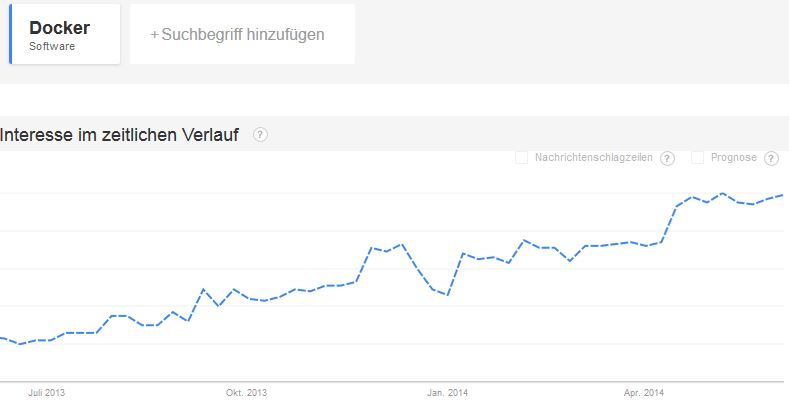
\includegraphics[scale=0.7]{img/docker_trend.JPG}\\
  \footnotesize\sffamily\textbf{Quelle:} \cite{google_trends_google_2014}
  \caption{Trend der Suchanfragen nach dem Begriff \grq Docker\grq\ im Bereich von 07.06.2013 - 07.06.2014 }
  \label{fig:google_trends}
\end{figure}

Schon innerhalb der ersten acht Monaten seit dem Start des Projekts wuchs die Zahl der beitragenden Personen auf über zweihundert an. 
Heute ist Docker bereits in namenhaften Projekten wie \grq Jenkins\grq , \grq Travis\grq\ oder \grq Vagrant\grq\ integriert. \cite{hykes_docker_2013}
Da Docker auf LXC basiert, hat es den großen Vorteil auf allen aktuellen Linuxsystemen ohne Änderungen zu laufen. Es erweitert LXC um eine benutzerfreundliche Schnittstelle zum erzeugen, verwalten und persistieren von Containern und übernimmt die Konfiguration der Inter-Container-
Kommunikation. Das ursprüngliche Ziel das Docker dabei verfolgt ist es Anwendungen mittels Containern in einen zuvor definierten, immer gleichen Kontext zu stellen. Die so in einen Container eingebetteten Anwendungen sollen dann unabhängig von der vorherrschenden Systemkonfiguration auf jedem beliebigen Hostsystem ausführbar sein.
Zum verwalten der Container setzt Docker auf einen Versionskontrollsystem ähnlichen Ansatz.
Neue Container werden immer ausgehend von einem bereits existierendem Stand gebildet und gespeichert. Änderungen an Containern werden damit sehr klein und sind dadurch besonders effizient zu übertragen.
Durch die Vereinfachung der Verwendung von LXC Containern öffnet Docker die Türe zu eine Vielzahl von möglichen Anwendungsszenarien die vor allem den Bereich des Cloud Computing vereinfachen und unterstützen können.
Die folgende Arbeit betrachtet eine Auswahl dieser Anwendungsszenarien.

\chapter{Architekturvarianten des Cloud Computing}
\label{cha:architekturvarianten_des_cloud_computing}
Cloud-Services werden üblicherweise in ein Schichtenmodell eingeteilt. Man unterscheidet dabei drei Schichten:
\begin{enumerate}
      \itemsep0pt
      \item Software as a Service (SaaS)
      \item Platform as a Service (PaaS)
      \item Infrastructure as a Service (IaaS)
\end{enumerate}
Die Zuteilung eines Services zu einer Schicht erfolgt anhand der Ebene im IT-Stack auf der der Service angesiedelt ist.
Die drei Ebenen lassen sich in einer Pyrmidenform darstellen. (siehe Abb \ref{fig:iaas_paas_saas}) 

\begin{figure}[htb]
  \centering  
  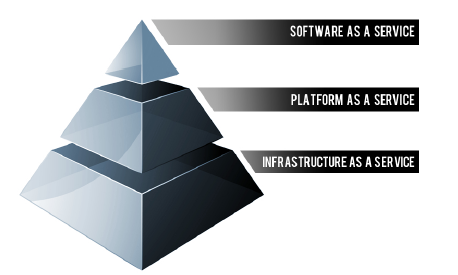
\includegraphics[scale=0.7]{img/iaas_paas_saas.png}\\
  \footnotesize\sffamily\textbf{Quelle:} \cite{kepes_understanding_????}
  \caption{Cloud Computing Architektur}
  \label{fig:iaas_paas_saas}
\end{figure}

Die höheren, abstrakten Schichten nutzen dabei die Dienste der tieferen, konkreten Schichten.
Docker kann die Cloud-Services vor allem in der Schicht Platform as a Service (PaaS) unterstützen.
Im folgenden werden die einzelnen Schichten kurz näher erklärt.
\section{Infrastructure as a Service (IaaS)}
\label{sec:iaas}
Die unterste Schicht bildet die Infrastructure as a Service-Schicht.
\glqq Diese Schicht stellt Mittel bereit, mit denen Basisspeicher und Rechenleistung als standardisirte Services über das Netzwerk angeboten werden können.\grqq \cite[S. 30]{meinel_virtualisierung_2011}
Anstelle sich Server, Speicherplatz und Netzwerk selbst zu kaufen, können Nutzer diese Resourcen
bei Bedarf von einem Infrastructure as a Service-Provider beziehen. Die Wartung und Pflege der Hardware kann so entfallen.
Dem Nutzer von Infrastructure as a Service wird eine Plattform bereitgestellt über die er volle Kontrolle hat. Diese Plattform ist dabei jederzeit skalierbar. Kurzzeitiger bedarf an zusätzlichen Hardware Ressourcen kann so kostengünstig ausgeglichen werden und muss nicht durch überschüssige, ungenutzte Hardware abgesichert werden.
Schwierige Planungen über den erwarteten Bedarf an Ressourcen können so entfallen und das Risiko einer Fehlplanung eliminiert werden.

\section{Platform as a Service (PaaS)}
\label{sec:paas}
Die mittlere Schicht bezeichnet man als Platform as a Service (Paas). In diese Schicht fallen Services die ein \glqq Programmiermodell und Entwicklungswerkzeuge bereitstellen, um Cloudbasierte Anwendungen zu erstellen und auszuführen.\grqq \cite{sommergut_faq_2014}
Der Nutzer des Services soll in der Lage sein, seine entwickelte Anwendung zu betreiben ohne sich dabei um die Rahmenbedingungen wie Hardware oder Software Infrastruktur kümmern zu müssen.
Der Platform as a Service-Provider liefert also alle nötigen Ressourcen wie Rechenleistung, Speicher und Netzwerk und skaliert diese abhängig von den Anforderungen der jeweiligen Anwendung.
Schwierige Aufgaben wie z.B. Loadbalancing werden dem Entwickler so abgenommen.
Platform as a Service setzt auf der darunterliegenden Schicht Infrastructure as a Service auf.
Auch bei Platform as a Service wird eine Infrastruktur bereitgestellt, diese wird aber noch um eine Ebene erweitert die es ermöglicht Webanwendungen schnell und einfach zu erstellen.

Unternehmen sind immer auf der Suche ihren Kunden einen Besseren Service und Support zu liefern.
Dabei wird in der heutigen zeit zumeist auf Webanwendungen gesetzt. Das Entwickeln und Betreiben dieser Anwendungen erweist sich allerdings oftmals als sehr zeitaufwendig und kostenintensiv.
Platform as a Service versucht dieses Problem zu lösen indem es den Entwicklern eine fertige Plattform anbietet. Die Entwickler können sich so ganz alleine auf die Entwicklung konzentrieren und müssen sich nicht um die gesamte Infrastruktur kümmern.

\section{Software as a Service (SaaS)}
\label{sec:saas}
Die höchste Schicht des Models bildet die Anwendungsschicht, die sogenannte Software as a Service-Schicht.
Software as a Service ist analog zu Platform as a Service zu betrachten. Hierbei wird jedoch keine Plattform zum entwickeln von Software über das Internet bereitgestellt, sondern die Software selbst. \cite{kepes_understanding_????}
Software as a Service ist der wohl bekannteste und am häufigsten genutzte Cloud Service. Die Nachfrage nach Software die nach diesem Modell bereitgestellt wird hat sich in den letzten Jahren rasant entwickelt. Dies ist vor allem den Komfort den Software as a Service bietet geschuldet.
Mit Software as a Service müssen sich Anwender nicht mehr mit ihrer eigen Hardware- und Softwareausstattung oder ihrem Betriebssystem auseinandersetzen wie sie es bisher gewohnt waren. Software wird ihnen einfach als Service über das Internet bereitgestellt.

Der Software as a Service \glqq Ansatz sieht vor, dass einzelne Softwarekomponenten bei einem Dienstleister betrieben werden, der allein für die gesamte Administration der Software verantwortlich ist, also Hardware und Software, Wartung und Betrieb. Dies betrifft auch die interne Ressourcenanpassung zur performanten Bereitstellung der Dienste.\grqq \cite[S. 34]{meinel_virtualisierung_2011}

Aus Unternehmenssicht werden dadurch Kosten gespart, da zeitaufwendige Aufgaben wie die Installation und Auslieferung der Software entfällt. Aufgaben wie das Aktualisieren werden von dem Software as a Service-Provider übernommen. Dadurch, dass die Software nicht mehr selbst verwaltet werden muss, sind neue Features oft sofort verfügbar und nicht erst mit dem nächsten Update-Zyklus der Unternehmens.
Darüber hinaus werden Software as a Service-Produkte oftmals nach der tatsächlichen Nutzung abgerechnet. Das ermöglicht es neue Plattformen ohne eine langfristige Bindung zu testen oder nur kurzzeitig zu nutzen.

\chapter{Anwendungen von Docker}
\label{cha:anwendungen_von_docker}
Docker ist eine Software die es ermöglicht Anwendungen zusammen mit ihren Abhängigkeiten in einen isolierten Container zu verpacken. Docker bedient sich dabei der Linux eigenen LXC-Conntainer Technologie und erweitert diese um eine simple Benutzer API (Application Pro-
gramming Interface) zum erzeugen, verwalten und für die Interaktion mit diesen Containern.
Die Eigenschaften von Docker können dabei wie folgt zusammengefasst werden \cite{abel_docker:_2013}:
\begin{itemize}
 
      \item \textbf{Dateisystem Isolation} \\
Jeder Prozess läuft in einem seperaten root-Dateisystem
      \item \textbf{Resourcen Isolation} \\
Systemressourcen wie CPU und Speicher können für jeden Container einzeln geregelt werden.
      \item \textbf{Netzwerk Isolation} \\
Jeder Prozess-Container läuft in seinem eigenen Netzwek-Namensraum mit einer seperaten, 			virtuellen Netzwekschnittstelle und IP-Adresse.
      \item \textbf{Copy-On-Write} \\
Änderungen am Dateisystem eines Containers weden in eine neue Schicht gespeichert und nicht in das originale Abbild übernommen. Dies erlaubt ein schnelles Anlegen neuer Container und spart sowohl Arbeits- als auch Festplattenspeicher.
      \item \textbf{Protokollierung} \\
Die Standard-Datenströme (stdout/stderr/stdin) jedes Containers werden protokolliert, um in Echtzeit oder als Stapel bearbeitet zu werden.
	  \item \textbf{Änderungsverwaltung} \\
Änderungen an Dateien in einem Container können zu einem neuen Abbild zusammengesetzt werden. Dieses kann als Grundlage für neue Container dienen.
	  \item \textbf{Interaktive Shell} \\
Docker kann ein Pseudo-Terminal anlegen und mit den Standard-Datenströmen verbinden, um eine interaktive Verbindung mit einem Container zu ermöglichen.
\end{itemize}
Docker wird seit März 2013 von der Firma dotCloud seit Oktober 2013 Docker
Inc.) unter der Apache Lizenz 2.0 veröffentlicht.\cite{github_dotcloud/docker_2013}
Im folgenden sollen mögliche Anwendungsfälle von Docker näher beleuchtet werden.
\section{Paas}
\label{sec:paas}
Die Firma dotCloud ist ein ein Platform as a Service-Provider. Als Erfinder und treibende Kraft hinter dem Docker-Projekt ist es also nicht verwunderlich, dass das Hauptanwendungsfeld von Docker im Bereich von Platform as a Service liegt.
Docker ist eigentlich eine Neuentwicklung eines Teils des Systems, welches sich dotCloud über die Jahre als 
Platform as a Service-Provider angeeignet hat. DotCloud verfolgt mit Docker das Konzept, einen Grundstein vorzugeben um den eine Platform as a Service-Infrastruktur aufgebaut werden kann.\cite[Zeit 18:24]{hykes_introduction_2013}

Um zu verstehen welche Vorteile Docker als Basis einer Platform as a Service-Infrastruktur bieten kann, muss man zunächst die Probleme betrachten, welchen sich ein Platform as a Service-Provider in der heutigen Zeit ausgesetzt sieht.

\subsection{Probleme von Paas}
\label{sec:probleme_von_paas}

Das Ausliefern von Code bzw. Software ist in der heutigen Zeit ein kompliziertes Unterfangen geworden. Aber wieso ist das so? Solomon Hykes, der gründer von dotCloud, sieht den Grund hierfür in den immer komplexeren Hardware- und Software-Stack mit denen wir uns in der heutigen Zeit konfrontiert sehen. \cite{hykes_introduction_2013} 
Vor nicht allzu langer Zeit bestand ein typischer Hardware- und Software-Stack noch aus einem simplen Server, dekoriert mit einer LAMP (Linux Apache MySQL PHP) Installation.
In den letzten Jahren haben sich jedoch sowohl der Hardware- als auch der Software-Stacks deutlich verkompliziert. (siehe Abb \ref{fig:hardware_software_stack}) 
\begin{figure}[htbp]
  \centering  
  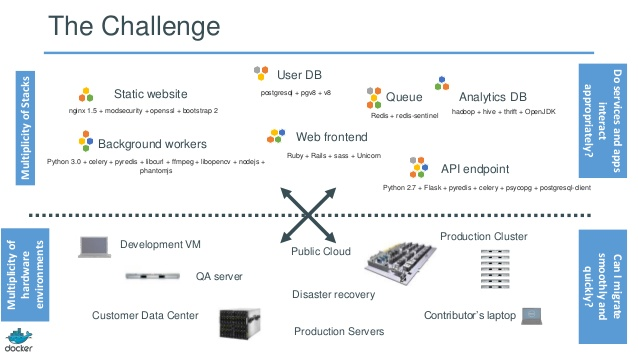
\includegraphics[scale=0.6]{img/hardware_software_stack.jpg}\\
  \footnotesize\sffamily\textbf{Quelle:} \cite{hykes_docker_2013}
  \caption{Unterschiedliche Hardware- und Software-Stacks}
  \label{fig:hardware_software_stack}
\end{figure}
Der Softwarestack reduziert sich nicht mehr auf eine simple Anwendung. Im Rahmen von Serviceorientierten Architekturen kommunizieren vielmehr viele verschiedene Stacks untereinander. Die einzelnen Stacks können sich dabei enorm unterscheiden was zum Beispiel die Programmiersprache oder die verwendeten Framewoks betrifft.
Plötzlich muss man nicht mehr nur einen einzelnen Software Stack isoliert betrachten sondern zusätzlich eine ganze Reihe von Services und deren Kommunikation untereinander.
Diese Vielzahl von Software-Stacks muss darüber hinaus auf einer immer komplexer werdenden Hardware-Infrastruktur betrieben werden. Entwickelte Software muss nicht mehr nur auf einem einzigen Server laufen sondern auf einer Vielzahl von unterschiedlicher Hardware wie z.b. Test-Server, Ernwicklungs-Pc, Laptop, Produktiv-Server etc.
Wir betreiben also einen immer komplexeren Software-Stack auf einer immer komplizierteren Hardware-Infrastruktur. Dabei muss sichergestellt sein, dass jeder einzelne Software-Stack auf jeder Infrastrukturkomponente betrieben werden kann und dabei immer das selbe Verhalten zeigt.
Das Ergebnis ist eine Matrix von Abhängigkeiten zwischen Software-Stacks und Hardware die mit jeder neuen Komponente rasant an Komplexität gewinnt.
Solomon Hykes bezeichnet diese Matrix als \glqq Matrix From Hell\grqq \cite[Zeit 4:30]{hykes_introduction_2013}(siehe Abb \ref{fig:matrix_from_hell}) 

\begin{figure}[htbp]
  \centering  
  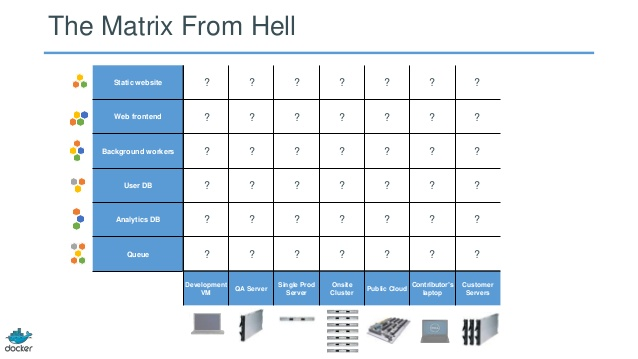
\includegraphics[scale=0.7]{img/matrix_from_hell.jpg}\\
  \footnotesize\sffamily\textbf{Quelle:} \cite{hykes_docker_2013}
  \caption{Matrix From Hell}
  \label{fig:matrix_from_hell}
\end{figure}

\subsection{Analogie mit der Frachtschifffahrt}
\label{sec:analogie_mit_der_frachtschifffahrt}
In der frühen Frachtschifffahrt sah man sich mit einem ähnlichen Problem konfrontiert und fand eine Lösung. Frachtschiffe müssen eine Vielzahl von Waren von einem Punkt A zu einem Punkt B transportieren. Analog zu unseren Software-Stacks können die Ware dabei völlig unterschiedliche Formen annehmen. Das Reicht beispielsweise von Autos über Elektronikgeräte bis hin zu kleinen Kaffeebohnen. All diese unterschiedlichen Gegenstände müssen auf ihrer Reise eine Vielzahl von Stationen analog zu unserer Hardware durchlaufen. (siehe Abb \ref{fig:waren_stationen}) 
\begin{figure}[htbp]
  \centering  
  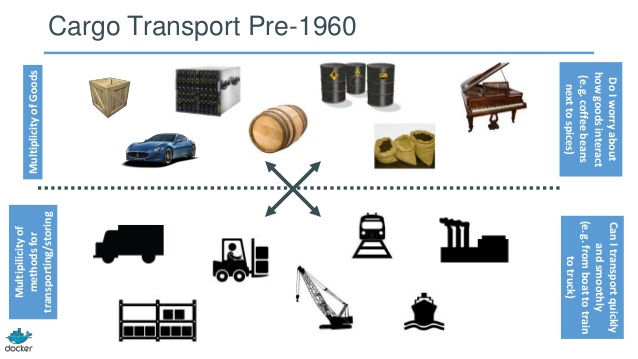
\includegraphics[scale=0.7]{img/waren_stationen.jpg}\\
  \footnotesize\sffamily\textbf{Quelle:} \cite{hykes_docker_2013}
  \caption{Waren und ihre Stationen in der Frachtschifffahrt}
  \label{fig:waren_stationen}
\end{figure}

Prinzipiell müssen dabei alle waren gleich behandelt werden. Auf Grund ihrer unterschiedlichen Beschaffenheiten ist dies jedoch nicht ohne weiteres möglich. Ein Auto muss zum Beispiel anders verladen werden als ein Sack Kaffeebohnen.
Kombiniert man wieder alle möglichen Waren mit allen Stationen die sie auf ihrer Reise durchlaufen müssen, ergibt sich ein ähnliches Bild wie in der \glqq Matrix From Hell\grqq Abb \ref{fig:matrix_from_hell}. (siehe Abb \ref{fig:waren_matrix_from_hell_ii}) 
\begin{figure}[htbp]
  \centering  
  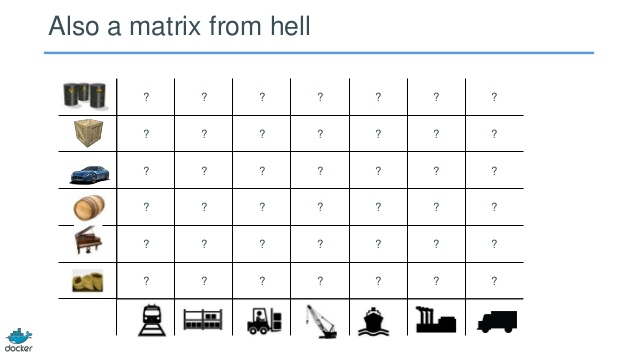
\includegraphics[scale=0.7]{img/waren_matrix_from_hell.jpg}\\
  \footnotesize\sffamily\textbf{Quelle:} \cite{hykes_docker_2013}
  \caption{Matrix From Hell II}
  \label{fig:waren_matrix_from_hell_ii}
\end{figure}

Die Lösung für dieses Problem ist der sogenannte Schiffscontainer. Alle Waren wenden bevor sie verschifft werden in einen einheitlichen, genormten Container verpackt. Die gesamte Infrastruktur kann sich somit auf ein einheitliches Format für zu verschiffende Waren standardisieren. Man schafft damit eine klare Trennung der Aufgabenbereich von Versender und Frachtschifffahrt. Die Infrastruktur muss sich nicht mehr darum kümmern wie einzelne Waren zu behandeln sind, sie verschifft nur noch Container und behandelt diese immer gleich. Der Versender der Waren hat sich hingegen nur noch darum zu kümmern, seine Güter in den Container zu verpacken. (siehe Abb \ref{fig:shipping_container})
\begin{figure}[htbp]
  \centering  
  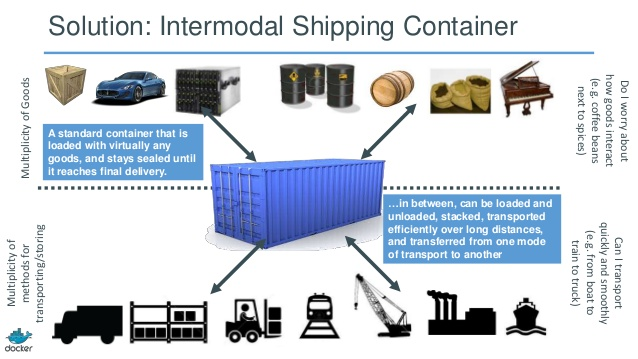
\includegraphics[scale=0.7]{img/shipping_container.jpg}\\
  \footnotesize\sffamily\textbf{Quelle:} \cite{hykes_docker_2013}
  \caption{Frachtcontainer}
  \label{fig:shipping_container}
\end{figure}

\subsection{Docker und Paas}
\label{sec:docker_und_paas}
Docker versucht genau dieses Konzept auf die Softwarewelt zu übertragen. 
Software wird nicht mehr einfach nur lose ausgeliefert sondern in einen standardisierten Container gepackt. Der Entwickler kümmert sich dabei um das Innenleben des Containers. Die Restliche Infrastruktur kümmert sich nur noch darum wie sie mit diesem Container umzugehen hat. Für beide Welten definiert Docker über ein klar spezifiziertes Interface die Spielregeln. (siehe Abb \ref{fig:container_fuer_code})
\begin{figure}[htbp]
  \centering  
  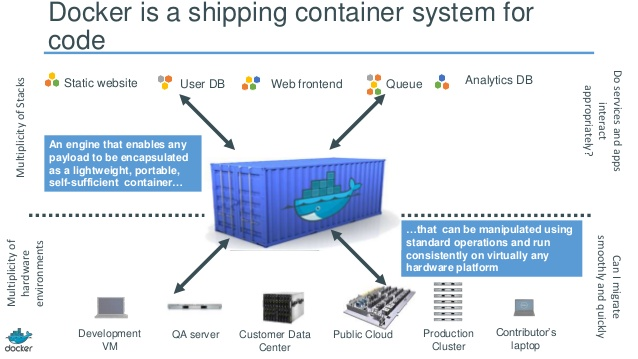
\includegraphics[scale=0.7]{img/hardware_software_container.jpg}\\
  \footnotesize\sffamily\textbf{Quelle:} \cite{hykes_docker_2013}
  \caption{Docker-Container für Code}
  \label{fig:container_fuer_code}
\end{figure}

Mit Hilfe von Docker ist es somit möglich die zuvor beschiedene \glqq Matrix From Hell\grqq Abb \ref{fig:matrix_from_hell} aufzulösen. Wird die Software in einer Standardisierten weise gekapselt kann sichergestellt werden, das die Abhängigkeiten zwischen den einzelnen Software-Stacks nicht verändert werden und immer gleich funktionieren. Sie sind sozusagen bereits vor der Auslieferung fest im Container verankert. Der Infrastruktur muss nur noch beigebracht werden mit einem Container umzugehen, nicht mehr aber mit vielen verschiedenen Software-Stacks. Das stellt jedoch kein größeres problem dar, da über das Standardisierte Interface die Schnittstellen bereits für alle Anwendungen gleich vorgegeben sind. (siehe Abb \ref{fig:aufgeloesste_matrix_from_hell})
\begin{figure}[htbp]
  \centering  
  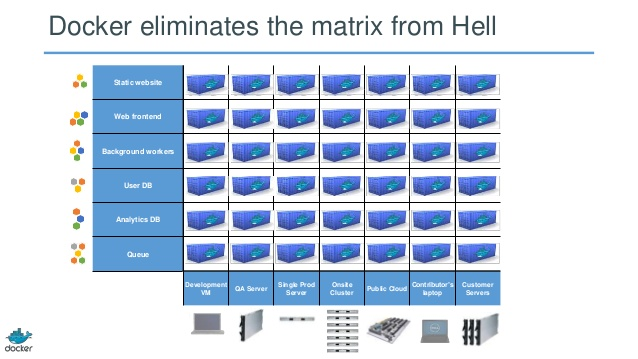
\includegraphics[scale=0.7]{img/aufgeloesste_matrix_from_hell.jpg}\\
  \footnotesize\sffamily\textbf{Quelle:} \cite{hykes_docker_2013}
  \caption{Aufgelößte Matrix From Hell}
  \label{fig:aufgeloesste_matrix_from_hell}
\end{figure}

Mit Hilfe von Docker ist es damit möglich einen großen Interessenskonflikt zwischen Platform as a Service-Provider und Platform as a Service-Nutzer zu beseitigen.
Der Nutzer möchte in der Regel eine möglichst große Freiheit. Er möchte selbst bestimmen wie die Abhängigkeiten seiner Software sind, welche Frameworks er verwendet oder in welcher Programmiersprache er seine Software implementiert. Er möchte sich nicht vorschreiben lassen unter welchen Rahmenbedingungen der seine Software umsetzt. Der Platform as a Service-Provider hingegen möchte möglichst kosteneffizient arbeiten und einen möglichst geringen Verwaltungsaufwand betreiben. Das bedeutet für ihn möglichst genaue Parameter festzulegen. Für ihn gibt es optimaler weise eine Programmiersprache, ein Framework so dass am ende alle auf der Plattform erzeugten Anwendungen gleich zu handhaben sind. Dieser Interessenskonflikt muss zwangsläufig in irgend einer Art von Kompromiss aufgelöst werden.
Eine für beide optimale Lösung wäre nach Solomon Hykes \cite[Zeit 13:50]{hykes_introduction_2013} die Verwendung von virtuellen Maschinen. Der Nutzer hätte die maximalst mögliche Freiheit beim Packen seiner Anwendung. Der Provider müsste sich nur auf das betreiben von virtuellen Maschinen spezialisieren. Dieses Konzept ist jedoch nicht praktikabel. Der Overhead an Daten wäre hierbei einfach viel zu groß. Im Grunde würde man für jede Anwendung immer einen komplette Rechner ausliefern. Darüber hinaus müsste man einige Einbußen im Bereich der Performance hinnehmen.
Mit Hilfe von Docker ist es möglich dies Lücke zu schließen. Innerhalb des Containers ist der Entwickler frei. Er kann hier also alle Parameter selbst so festlegen um sicherzustellen, dass die Anwendung die er lokal sich auf der Inrastruktur des Platform as a Service-Providers noch genauso verhalten wird. Gleichzeitig ist der Overhead an Daten und der Pervormanceverlust eines Docker Containers so gering, dass er kein Argument mehr gegen seine Verwendung darstellt.
Docker bildet somit die Optimale Basis um darum einen effizienten Platform as a Service aufzubauen. 

\section{Saas}
\label{sec:saas}
Die grenzen zwischen Platform as a Service und Software as a Service sind fliesend.
Verwendet man Docker wie bereits im Abschintt \ref{sec:docker_und_paas} gezeigt als Kern einer Platform as a Service-Umgebung, um darauf wiederum Software bereitzustellen, verwendet man Docker im Grunde bereits zum Betreiben von Software as a Service.

\subsection{Docker und Saas}
\label{sec:docker_und_saas}
Docker kann darüber hinaus jedoch auch explizit zur Implementierung einer Software as a Service Lösung verwendet werden. Jede Instanz der angebotenen Softwarelösung wird dabei in einen eigenen Container verpackt. Mit Hilfe eines sogenannten \grq Dockerfiles\grq\ kann das Innenleben eines Containers genau definiert werden. Ein Dockerfile enthält dazu eine Reihe von Dockerbefehlen die später sequentiell ausgeführt werden sollen. Compiliert man ein solches Dockerfile entsteht daraus ein Abbild des gewünschten Systems welches als \grq Dockerimage\grq\ bezeichnet wird.
Dieses Image kann nun verwendet werden um beliebig viele immer gleiche Instanzen in Form von \grq Docker Containern\grq\ zu erzeugen.
Hier wird klar wie Docker das Anbieten einer Software mittels Software as a Service unterstützen kann.
Die gewünschte Software muss nur einmal innerhalb eines Dockerimage definiert werden. Für jeden Benutzer der eine Instanz der Software as a Service-Lösung benötigt muss also nur noch ein eigener Container aus diesem Image erzeugt werden. Alles was man also neben einem funktionsfähigem Image noch benötigt um eine Software als Software as a mit Hilfe von Docker anzubieten ist eine Webanwendung die das erzeugen, verwalten und Bereitstellen der Container für die einzelnen Benutzer übernimmt.
Ein mögliches Anwendungsgebiet wäre es zum Beispiel Nutzern auf einfache und unkomplizierte Art und weise Testinstanzen eine neuen Software bereitzustellen um diese einmal auszuprobieren und somit das Eigene Produkt zu vermarkten.
Juien Barbier hat eine Beispielanwendung erstellt die zeigen soll, dass dieses Konzept auch in der Praxis umgesetzt werden kann.
In seinem Projekt \glqq Build Your Own SaaS with Docker\grqq \cite{barbier_build_2013} hat er eine einfache Webanwendung erstellt mit deren Hilfe Docker Container erzeugt und bereitgestellt werden können. Mit seiner Anwendung ist es möglich den Cache-Server \grq Memcached\grq\ als Software as a Service über das Internet anzubieten. Mit wenigen Mausklicken können sich Benutzer eine eigene Memcached Instanz erzeugen und diesen über das Internet ansprechen.
Im Hintergrund wird dafür aus einem vordefinierten Image ein neuer Docker Container mit einer laufenden Memcached-Instanz erzeugt.
Paul Czarkowski hat in einer ähnlichen Anwendung mit dem selben Vorgehen einen  IRC Bouncer als Software as a Service erstellt. Dabei hat er gezeigt, dass selbst mit einem Server mit nur 512 mb Hauptspeicher das betreiben von einhundert gleichzeitigen Instanzen Problemlos möglich ist.
Mit Hilfe von Docker kann man also auf recht simple Art und Weise eine Vielzahl von unterschiedlichen Anwendungen als Software as a Service zu betreiben.

\chapter{Secure Sandboxes}
\label{sec:secure_sandboxes}
Chapter behandelt: Die verwendung von Docker als sichere Sandbox.
\section{Sicherheit von Containern}
\label{sec:sicherheit_von_containern}
Wie steht es um die Sicherheit eines Dockercontainers.

\subsection{Anwendungsrepository}
\label{subsec:anwendungsrepository}
Einsatzmöglichkeit des Containers als sichere Sandbox

\section{Dependencyinjection für Systemumgebungen}
\label{sec:sicherheit_von_containern}
Einsatzmöglichkeit des Containers als "Dependencyinjection für Systemumgebungen" wie sie z.B oft bei automatisierten Tests in der Softwareentwicklung benötigt werden.


%Verzeichnis aller Bilder
\newpage
\listoffigures

%Literaturverzeichnis
\newpage
\bibliographystyle{alphadin}
\bibliography{Literatur}

\end{document}
